\documentclass{mc2015}

%%%%%%%%%%%%%%%%%%%%%%%%%%%%%%%%%%%%%%%%%%%%%%%%%%%%%%%%%%%%%%%%%%%%%
\usepackage[T1]{fontenc}         % Use T1 encoding instead of OT1
\usepackage[utf8]{inputenc}      % Use UTF8 input encoding
\usepackage{microtype}           % Improve typography
\usepackage{booktabs}            % Publication quality tables
\usepackage{amsmath}
\usepackage{graphicx}
\usepackage{float}
\usepackage{wrapfig}
\usepackage[exponent-product=\cdot]{siunitx}
\usepackage[colorlinks,breaklinks]{hyperref}
\hypersetup{linkcolor=black, citecolor=black, urlcolor=black}

\usepackage{lipsum}

\def\equationautorefname{Eq.}
\def\figureautorefname{Fig.}

%%%%%%%%%%%%%%%%%%%%%%%%%%%%%%%%%%%%%%%%%%%%%%%%%%%%%%%%%%%%%%%%%%%%%
% Insert authors' names and short version of title in lines below

\authorHead{B.S. Cornille}
\shortTitle{Shared Memory MC}

%%%%%%%%%%%%%%%%%%%%%%%%%%%%%%%%%%%%%%%%%%%%%%%%%%%%%%%%%%%%%%%%%%%%%
\begin{document}

\title{Shared Memory Monte Carlo with MPI+MPI}

\author{Brian Cornille}
%\author{Author B\footnote{Footnote, if necessary}}
\affil{University of Wisconsin-Madison \\
%  1500 Engineering Dr. \\
%  Madison, WI 53706 \\
  bcornille@wisc.edu}

%\author{Author C}
%\affil{
%  Department of Nuclear Engineering \\
%  Name of University \\
%  Address \\
%  C@name.univ.edu
%}

\maketitle

\begin{abstract}



\emph{Key Words}: Monte Carlo, MPI+MPI
\end{abstract}

%%%%%%%%%%%%%%%%%%%%%%%%%%%%%%%%%%%%%%%%%%%%%%%%%%%%%%%%%%%%%%%%%%%%%
\section{Introduction}



\subsection{Motivation for Shared Memory}



\subsection{Shared Memory Programming Considerations}



\subsubsection{MPI\_Accumulate}



\subsection{Model Problem}

A very simple model problem was desired for this study.
Since no physics was to be tested, it was not necessary to model a
physically realistic test case.
The only requirement for the test problem was that an appropriate amount
of computation should be done between each particle transport step.

\subsubsection{Geometry}

The model geometry was chosen to be a single cell with the shape of a rhombicuboctahedron.
A rhombicuboctahedron has 26 faces, of which 18 are square and 8 are equilateral triangles
(see \autoref{fig:shape}).
This shape was chosen for having many unique bounding surfaces that are simple to define.
Having many bounding surfaces adds computation when determining the next particle position.
This helps the model problem approximate the computational time
per particle transport step of a realistic case.

\begin{wrapfigure}{R}{0.47\textwidth}
	\centering
		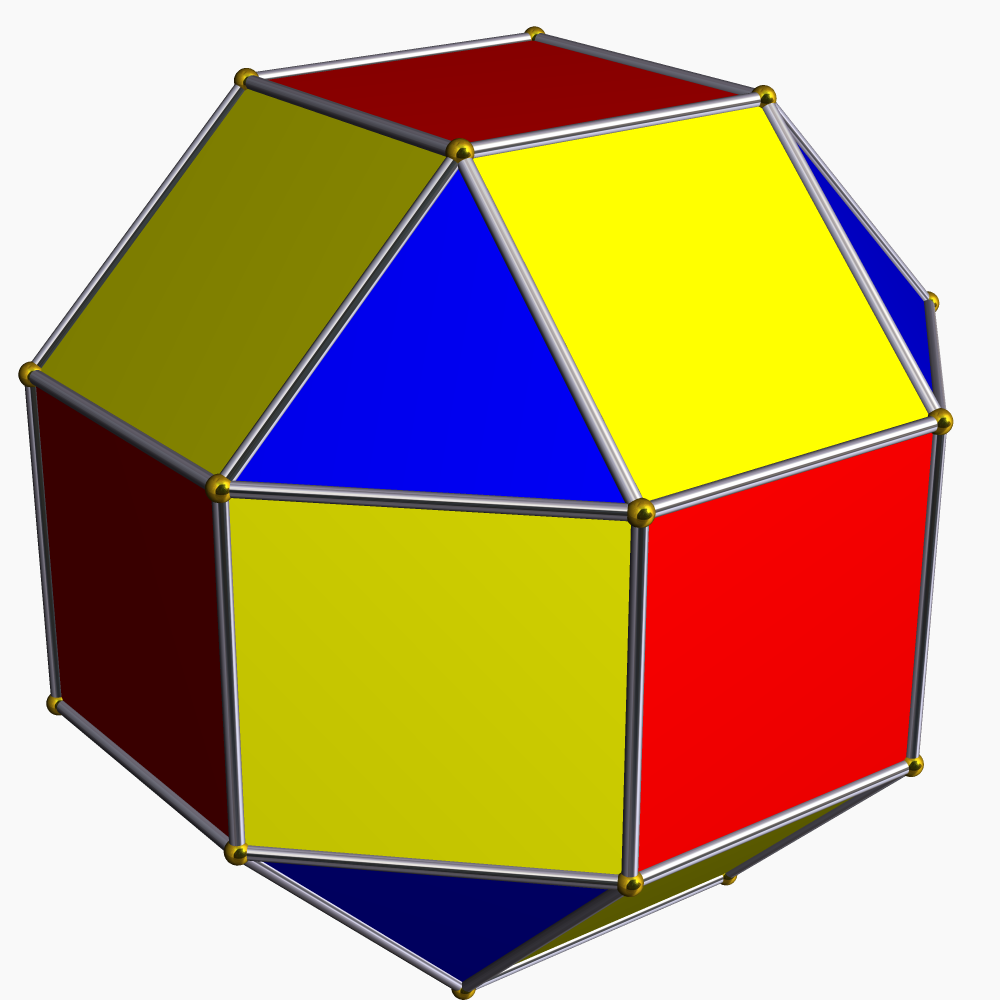
\includegraphics[width=0.35\textwidth]{Small_rhombicuboctahedron.png}
		\caption{\small "Small rhombicuboctahedron" by Tomruen -
			\url{http://en.wikipedia.org/wiki/Image:small_rhombicuboctahedron.png.}}
		\label{fig:shape}
\end{wrapfigure}

\subsubsection{Material properties}

A made up 

\subsubsection{Tally}



%%%%%%%%%%%%%%%%%%%%%%%%%%%%%%%%%%%%%%%%%%%%%%%%%%%%%%%%%%%%%%%%%%%%%
\section{Conclusions}

\begin{figure}[h]
	\includegraphics[width=\textwidth]{timings.pdf}
\end{figure}

%%%%%%%%%%%%%%%%%%%%%%%%%%%%%%%%%%%%%%%%%%%%%%%%%%%%%%%%%%%%%%%%%%%%%
\section{Acknowledgments}



%%%%%%%%%%%%%%%%%%%%%%%%%%%%%%%%%%%%%%%%%%%%%%%%%%%%%%%%%%%%%%%%%%%%%
\setlength{\baselineskip}{12pt}

\bibliographystyle{mc2015}
\bibliography{references}

%%%%%%%%%%%%%%%%%%%%%%%%%%%%%%%%%%%%%%%%%%%%%%%%%%%%%%%%%%%%%%%%%%%%%
\appendix
\section{}


\end{document}
